El método de reducción también es adaptado del presentado por Abdolhosseinzadeh \citep{Abdolhosseinzadeh2015}. Éste es un método de reducción química, y se realiza en solución acuosa.

\section{Materiales}
Como precursor se usa el óxido de grafeno sintetizado con anterioridad mediante el método modificado de Hummers. Como agente reductor se utiliza en primera instancia ácido ascórbico (\ce{C_6H_8O_6}, Sigma-Aldrich $>$95\%).

\section{Procedimiento}
En primer lugar, 30 g de ácido ascórbico se disuelven en 300 ml de agua destilada, para ser agregados a una de las parte de óxido de grafeno obtenido anteriormente bajo agitación (aproximadamente 300 ml de solución). Al añadir el ácido ascórbico ya en solución, la mezcla se vuelve negra gradualmente, esta es una señal de que la reducción se está llevando a cabo, además, la mezcla deja de ser heterogénea, signo de la hidrofobicidad del rGO. En una primera síntesis, la mezcla es llevada a 90 \degree C y se mantiene por 1 hr dentro del rango de temperatura 85-95 \degree C. También se realizan reducciones a otras temperaturas, sean, 65 \degree C, temperatura ambiente, en baño de hielo.

\section{Resultados}
Los materiales obtenidos son caracterizados por espestroscopia de rayos x (XRD), UV-Vis, y microcopia SEM.

\begin{figure}
	\centering
	\fbox{
		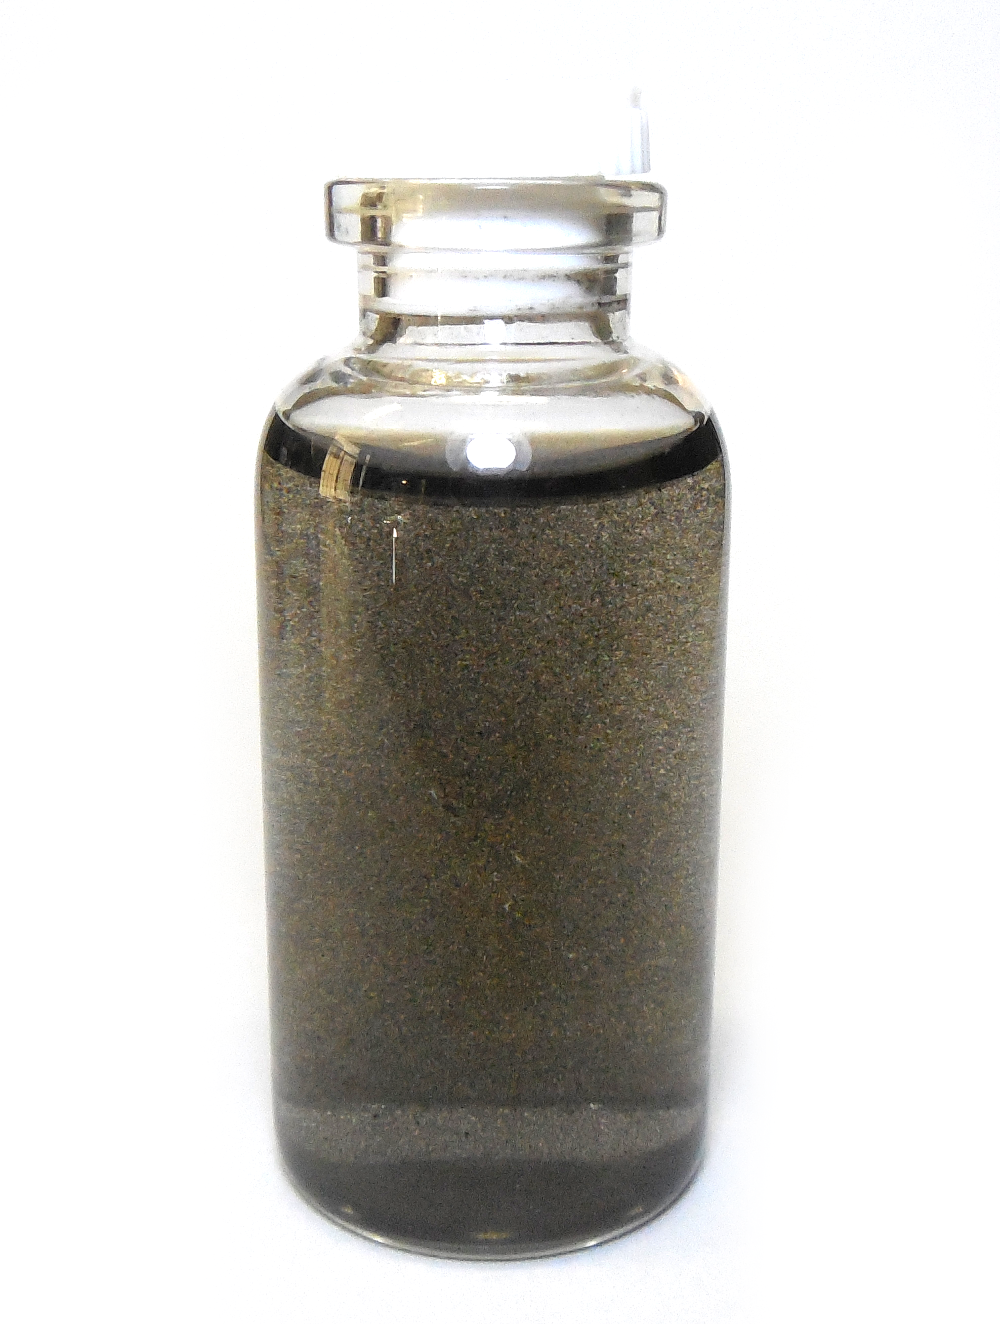
\includegraphics[width=0.5\textwidth]{RGO_pic.png}
		}
	\caption{RGO}
	\label{fig:RGO}
\end{figure}
